
\chapquote{``Please, Oh please, publish me in your collection of self-referential sentences!"}{Douglas Hofstadter}

\problem A \textit{quine} is a non-empty computer program which takes no input and produces a copy of its own source code as its only
output.

Write a \textit{quine} in \textit{Java}.


\textit{(Note that a program which finds its source code file and displays it is not considered a \textit{quine}, since it takes a file as input.)}

\solution
\begin{figure}[h]
	\begin{center}
		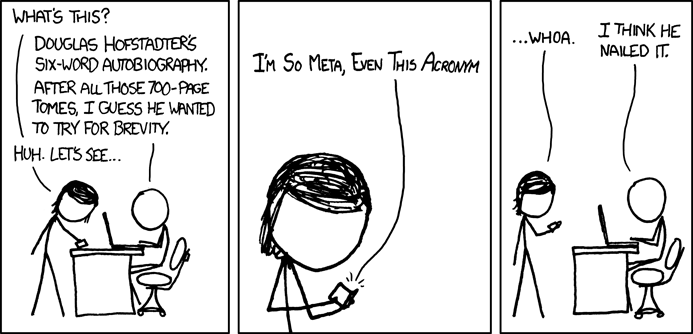
\includegraphics[scale=0.5]{hofstadter.png}
	\end{center}
	\caption*{Hofstadter (\texttt{xkcd.com/917})}
	\label{fig:xkcd_hofstadter}
\end{figure}

The name \textit{quine} was coined by \textit{Douglas Hofstadter} in his brilliant book \textit{G\"odel, Escher, Bach: An Eternal Golden Braid}, in
honour of the philosopher \textit{Willard Van Orman Quine}, who extensively studied indirect self reference, in particular the following
statement known as \textit{Quine's paradox}.
\begin{quote}
	``Yields falsehood when preceded by its quotation" yields falsehood when preceded by its quotation.
\end{quote}

Although writing a \textit{quine} in \textit{Java} seems impossible at first glance, it can be shown that \textit{quines}
exist in any \textit{Turing complete} programming language.

We might start off by writing the following code.
\lstinputlisting{QuineA.java}
A problem arises --- what can we write in place of \texttt{???} ? This part of the string must contain the entire string itself.
Is this possible without the string being infinitely long?

The problem is that the string we seek must contain the characters to be printed, and also be able to be used to print itself.
The following code snippet illustrates this.
\lstinputlisting{QuineB.java}
What can replace \texttt{???} so that the entirety of line 1 is displayed?

A solution is as follows.
\lstinputlisting{QuineC.java}

We can now use this template to move the entirety of the code into the string, including the print statement itself. This leads to another problem
--- double quotes are now inside double quotes, and must be escaped (\texttt{\textbackslash"}). However, the backslashes themselves will not appear
in the output. This can be solved by using the ASCII value for an double quote, which is \texttt{34}, in place of an escaped double quote.
Discarding newlines and delcaring the string \texttt{s} as a global variable at the very end of the program minimizes the amount of code
considerably.

The result is the following \textit{quine}.

\lstinputlisting{src/Quine.java}

\varDescription
\begin{longtable} {| >{\ttfamily}p{0.16\linewidth} | >{\ttfamily}p{0.2\linewidth}| p{0.6\linewidth} |}
\hline\multicolumn{3}{|c|}{\tt Quine} 		\\\hline
String		&	s		&	Stores the entire source code of the program \\\hline
\hline\multicolumn{3}{|c|}{\tt Quine::main()} 		\\\hline
char		&	q		&	Stores a double quote	\\\hline
\end{longtable}
